\documentclass{IEEEtran}
\usepackage{cite}
\usepackage{amsmath}
\usepackage{graphicx}
\graphicspath{{images/}}
\begin{document}
\title{A Review on Neural Language Modeling}

\author{Anuar Maratkhan}

\maketitle

\section{Introduction}

Language Modeling (LM) is a central task in Natural Language Processing (NLP) and play main role in speech recognition, machine translation, optical character recognition, natural language understanding, question answering and many other tasks. Language modeling is all about sequential data. \textit{Language model} is an algorithm for predicting next word in a text given preceeding ones. It is also mostly known as \textit{statistical language model} for its richness in statistical approaches in previous works. The state-of-the-art statistical language models turned up to be cache models and class-based models. In addition, according to \cite{Mikolov2010NeuralLM}, most of the statistical models require more data for better performance. 

However, as soon as neural networks became popular, \textit{neural language modeling} approaches were invented. Artificial neural networks perform well on supervised learning tasks (when the data is \textit{labeled}) and unsupervised learning tasks (when the data is \textit{unlabeled}). Quoc V. Le, et al. in their study \cite{unsupervised} explored and demonstrated how well neural networks operate on unsupervised learning task, where a model has to detect whether the given image contains face or not. And as the study \cite{unsupervised} notes, the work has been motivated by neuroscience hypothesis. So does the whole science about neural networks. Moreover, information retrieval tasks that are mainly composed of unlabeled data ,like in search engines, can be approached by such unsupervised learning techniques. Neural language models, also known as continous-space language models, make use of these neural networks. These are current state-of-the-art approaches in language modeling.

% NOT SUFFICIENT PART
This part of the introduction will conclude earlier approaches to language modeling, particularly statistical ones that are \textit{unigram}, \textit{bigram}, \textit{trigram}, and more generalized \textit{N-gram} models. (DO WE REALLY NEED IT?)
% NOT SUFFICIENT PART

In the second section of this paper we start by reviewing Recurrent Neural Networks (RNN). Further, in the same section we review the first/previous and current state-of-the-art RNN based word-level language modeling approaches, starting from \cite{Mikolov2010NeuralLM} and \cite{Mikolov2011ExtensionsOR}, proceeding by \cite{Zaremba2014LSTM}, and \cite{Salakhutdinov2017Softmax}. Next section presents different approaches on neural language modeling that include division of words into subwords presented in \cite{Mikolov2011SubwordLM}, reinforcement learning based techniques from \cite{}, and neural Turing machines approach \cite{}.

\section{Recurrent Neural Networks based Language Models}

\subsection{Recurrent Neural Network}

Recurrent Neural Networks (RNN) are primarily used in sequential data analysis such as video processing, text processing, predicting stock prices. RNN architecture is an improvement of feed-forward networks that takes into account previous hidden layer results by storing them in memory. An invention of backpropogation caused an exciting use of RNNs \cite{deeplearning}.

Simple recurrent neural network used in \cite{Mikolov2010NeuralLM} can be described by input at time \(t\) --- \(x(t)\), hidden layer at time \(t\) --- \(s(t)\), and the output layer at time \(t\) --- \(y(t)\), which are computed as follows:

\begin{equation}
	x(t) = w(t) + s(t-1)
\end{equation}
\begin{equation}
	s_j(t) = f\Bigg(\sum_i{x_i(t)u_ji}\Bigg)
\end{equation}
\begin{equation}
	y_k(t) = g\Bigg(\sum_j{s_j(t) v_kj}\Bigg)
\end{equation}

where (1) uses current word at time \(t\) and preceeding/previous hidden layer at time \(t-1\) as input, (2) and (3) have weights \(u\) and \(v\) used for computations, and both also have sigmoid activation function and softmax function, which are:

\begin{equation}
	f(z) = \frac{1}{1+e^{-z}}
\end{equation}
and
\begin{equation}
	g(z_m) = \frac{e^{z_m}}{\sum_k{e^{z_k}}}
\end{equation}
respectively.

The problem of simple RNN is that the backpropogated gradients vanshish or explode \cite{rnn}. Therefore, the improvement in RNN architecture further was introduced with invention of Long-Short Term Memory (LSTM). The LSTM solved the vasnishing gradient problem by having special cells with activation gates. Moreover, Gated Recurrent Unit (GRU) improved the architecture of the LSTM by combining two gates. The study shows that RNNs perform better than complex statistical approaches, N-grams, on a real-world data \cite{rnn}.

\subsection{Language Models}

Neural language models have demonstrated relatively superior performance on language modeling and speech recognition tasks in comparison to the state-of-the-art statistical approaches, class-based models, in the last decades. Neural models take their first steps from taking the advantage of feed-forward networks that are listed in \cite{Mikolov2010NeuralLM}, which motivated T. Mikolov, et al. to investigate the performance of more advanced type of neural network, RNN. The study was first to evaluate RNN for modeling such sequential data.

In contrast to feed-forward networks that use fixed size of context to predict next word in a sequence, RNNs does not require to use limited number of preceeding words \cite{Mikolov2010NeuralLM}. The structure of simple recurrent neural network used in the study is shown in Fig. \ref{fig:rnn} below.

\begin{figure}[h]
	\centering
	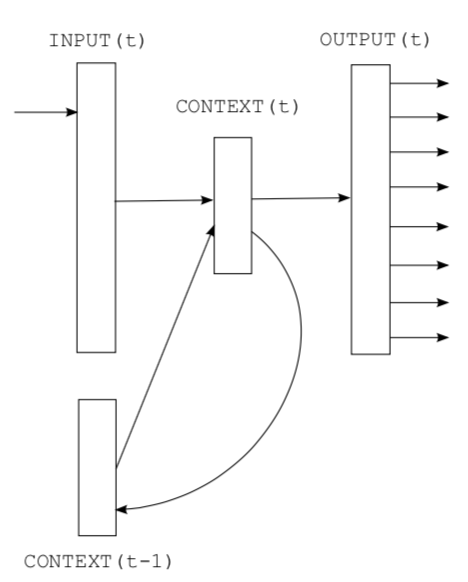
\includegraphics[width=0.3\textwidth]{rnn}
	\caption{Simple recurrent neural network from \cite{Mikolov2010NeuralLM}}
	\label{fig:rnn}
\end{figure}


\section{Subword-level Language Modeling}

This section will show how subword language modeling exceeds the performance of word-level and characted-level language modeling by presenting previous approaches from \cite{Mikolov2011SubwordLM}, etc...

\section{Reinforcement Learning}

This section will show some Reinforcement Learning (RL) approaches to language modeling tasks and applications such as dialogue systems, machine translation, text generation.

\section{Neural Turing Machines}

This section will discuss Neural Turing Machines (NTM) approach to different natural language processing tasks with controllers like feed-forward network, GRU, LSTM, and further will show applications in learning language models. Related papers are \cite{snips16}, etc...

\section{Conclusion}

Over the past few years, it was clearly seen that continous-space language models outperformed statistical modeling techniques significantly. The ease of feature learning without need in extraction of those features simplified lives of scientists. The neural approach offers such opportunity to its users.

Recurrent networks are expected to improve natural language understanding in real-world applications.

To be continued...


\bibliographystyle{IEEEtran}
\bibliography{reference}
\printbibliography

\end{document}